\section{Architecture}

Modern computer science emphasize parallelism as a highly important property in
order to achieve speed on multicore processors. As the size of the log files
which PET has to parse can easily be 10s of gigabytes large, PET has to be
designed with performance in mind. This means that PET must be lightweight and parallel
in order to be fast, while it must maintain correctness and be easy to use.

Due to memory constraints on commonly available computers, it is not feasible to read the entire log
file into memory and then start parsing. It would also make the reading step a serial part of the program,
which hinders parallelism. It will also be a bad idea to read one line, parse
it, weight it and apply it to the grand total, as it would be an entirely serial process.

\subsection{Overview}

\begin{figure}[ht]
    \includegraphics[width=0.9\textwidth]{figs/pet-pipeline-gv.pdf}
    \caption{How PET works}
    \label{fig:pipeline}
\end{figure}

In order to maintain good speed while still keeping the PET source code
readable, PET has been implemented using ideas from the producer-consumer scheme
as explained by Gamma et.  al.  in\cite{designpatterns}. As depicted in
\autoref{fig:pipeline}, this scheme makes it rather easy to let a producer read
the lines from the log file into a ring buffer and let multiple consumers pick
from this ring buffer. Each consumer parses the log lines they pick, and apply
the weight of each read event to each their result vector. When all lines are
read and parsed, the results vectors are merged, and idle-task power and static
power consumption is added.

\subsection{Details}


\autoref{fig:callgraph}


PET is a tool which main task will be to 

When designing a tool for parsing large input files and applying flexible configuration alternatives,
there are quite a few aspects that needs to be considered. Through this section the design choises
briefly explained in \autoref{sec:whatispet} will be further explained and more deeply understood.

PET has to be designed for good performance.


\begin{figure}
%    \includesvg[clean,eps,pretex=\relscale{0.25},width=\textwidth]{figs/maincallgraph}
    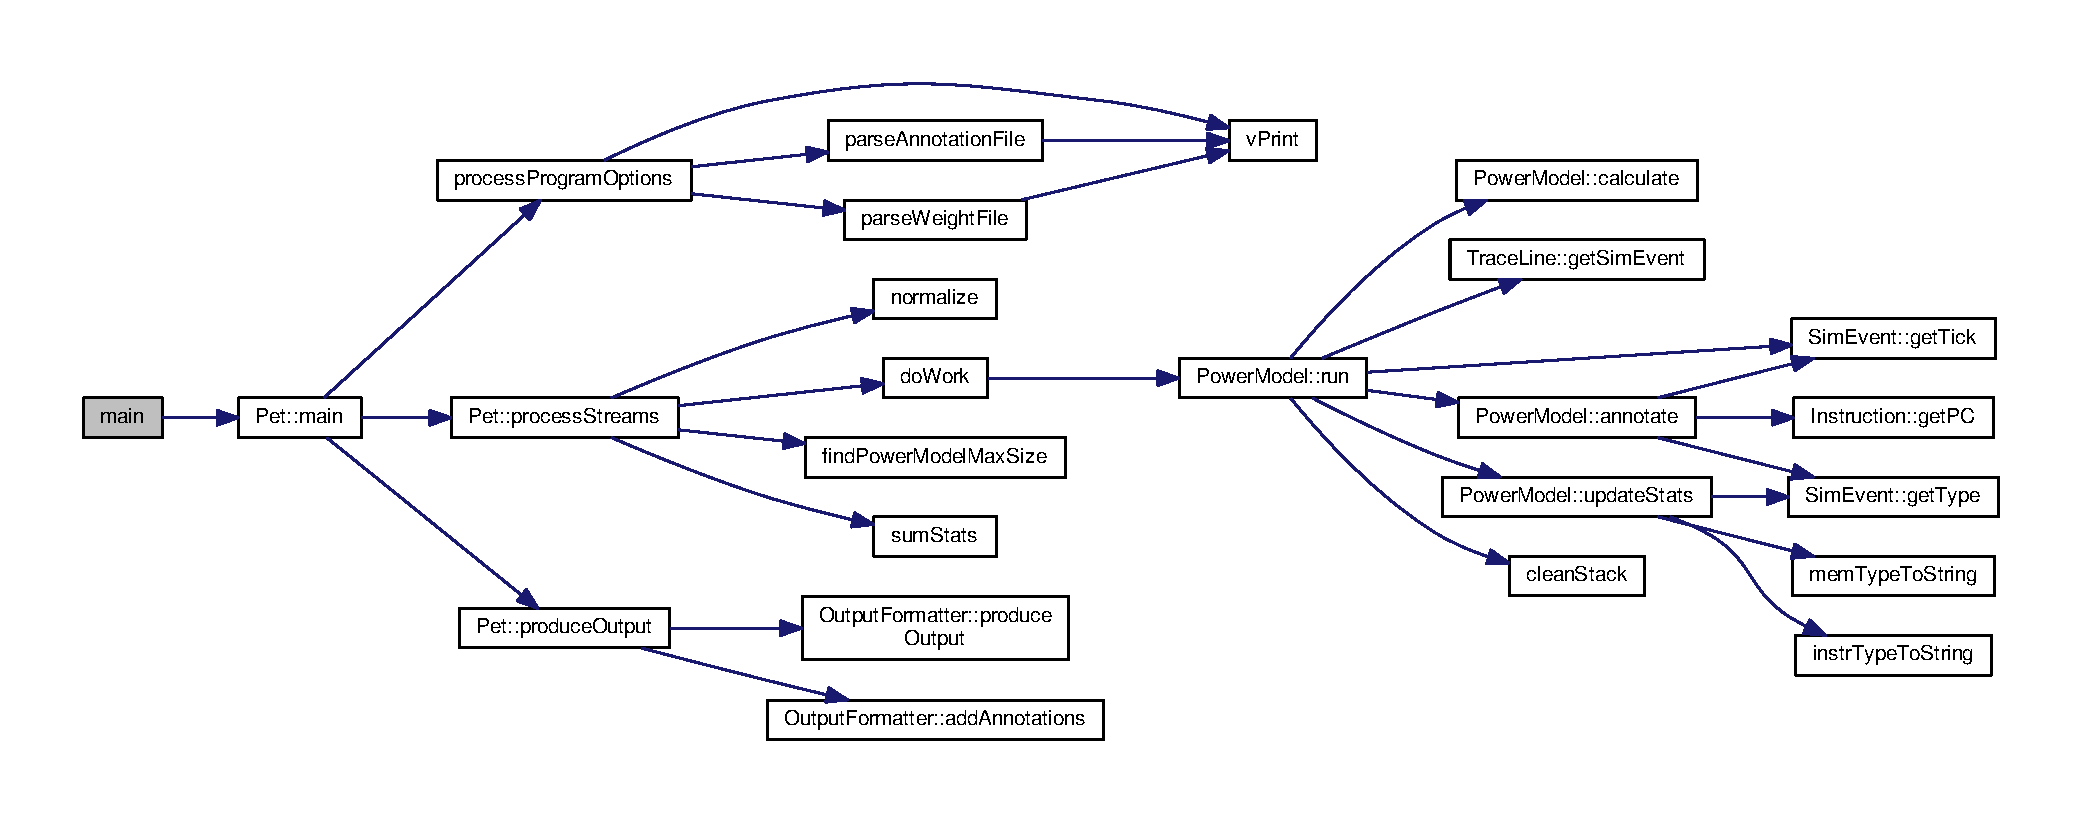
\includegraphics[width=\textwidth]{figs/maincallgraph.pdf}
    \caption{Call graph}
    \label{fig:callgraph}
\end{figure}

put UML-figures here
trådpool
concurency
arbeidsdeling
ringbuffer, statisk vs. ikke statis størrelse




